\documentclass[11pt]{article}
\usepackage[margin=1in]{geometry}
\usepackage[T1]{fontenc}
\usepackage{lmodern}
\usepackage{microtype}
\usepackage{amsmath}
\usepackage{booktabs}
\usepackage{tabularx}
\usepackage{xcolor}
\usepackage{pgfplots}
\pgfplotsset{compat=1.18}
\usepackage{enumitem}
\setlist{itemsep=2pt,topsep=4pt}
\usepackage[hidelinks]{hyperref}

\newcommand{\code}[1]{\texttt{#1}}

\title{Exact, Output-Identical Acceleration of MAFFT\\on Apple Silicon and x86}
\author{Claude Code (Claude Opus 5.5, Anthropic)\thanks{Claude Code, running Claude Opus 5.5,
designed, implemented, verified and benchmarked the optimizations and wrote this report.
Josh Walker advised and set the research direction.} \and Josh Walker}
\date{Technical report, September--October 2026}

\begin{document}
\maketitle

\begin{abstract}
We describe five successive builds of the multiple sequence aligner MAFFT (v7.525/7.526),
the first four optimized for an Apple M1 machine and the fifth for x86-64 servers. The
constraint throughout was that output must be \emph{byte-identical} to unmodified MAFFT, so
that downstream analyses calibrated on stock output are unaffected. The first round (opt1)
found that much of the run time in the accurate L-INS-i mode went not to the
dynamic-programming (DP) recurrences but to bookkeeping, and removed it with algorithmic
fixes, NEON vectorization, and matrix products run through Accelerate on the M1's AMX units.
The second round (opt2) measured how iterative refinement behaves on this data --- about 85\%
of refinement steps reproduce the current alignment --- and added a pair-score cache, a fully
vectorized prefix scan, and run-based column counts. The third build (opt3) moves the
all-pairs local-alignment stage to the M1 GPU with an integer Metal kernel that reproduces
MAFFT's recurrence, tie rules and traceback exactly. The fourth (opt4) compiles that shader
at build time and retunes it for GPU occupancy. On a production phylogenetics workload of
fungal ITS alignments, opt4 runs L-INS-i 6.5$\times$ faster than stock MAFFT 7.526 in a
single run (7.2$\times$ less CPU) and 4.6$\times$ faster at the production setting of 8
concurrent alignments.

The fifth build (opt5) ports the vector kernels to AVX-512 for AWS instances and leaves the
arm64 machine code unchanged. On c7i and c7a instances it runs L-INS-i 5.7--7.0$\times$
faster than stock in a single run and 5.1--5.9$\times$ faster at four concurrent alignments,
and a c7a.xlarge aligns about 820 production shards per hour. Porting
exposed a fact that matters more than the speed: \emph{stock MAFFT itself} does not give the
same alignments on every platform. A gcc build on x86 disagrees with the Mac on 33\% of
inputs, because Apple's clang fuses multiply-adds into a single rounding and gcc does not.
A clang build with FMA on x86 reproduces the Mac's alignments on all 181 inputs tested, on
Intel and AMD alike; it became the reference for the production deployment, with opt5
verified against it. Every output of every build in every test was byte-identical to its
stock reference, across all tested strategies and more than 5{,}000 production alignments
checked end to end. The one discrepancy the rewrite introduced, a rounding difference, was
caught by independent validation and fixed.
\end{abstract}

\section{Introduction}

MAFFT~\cite{katoh2002,katoh2013} is among the most widely used multiple sequence aligners.
Its iterative-refinement modes with pairwise alignment information, notably L-INS-i and
G-INS-i~\cite{katoh2005}, are considerably more accurate than its progressive modes, but
also much slower. This work was prompted by a concrete cost: a phylogenetics pipeline
(``seqhesion'') aligns 2{,}415 fungal ITS barcode sets per genomic region with L-INS-i, at
roughly 80--95\,s each, and MAFFT is about 99\% of the pipeline's run time.

Faster aligners exist, but they change the answer. The pipeline's own measurements, taken
by comparing well-supported splits of FastTree~\cite{price2010} trees built after
trimAl~\cite{capella2009} trimming, found that MAFFT FFT-NS-1 (135$\times$ faster) recovers
78.3\% of the splits supported in the L-INS-i trees, and spoa~\cite{vaser2017} recovers
69.7\%. We therefore set a stricter goal: make L-INS-i faster \emph{without changing a single
output byte}. Such a speedup costs nothing in accuracy and needs no revalidation downstream.

The work proceeded in five builds, each installed only after verification
(Table~\ref{tab:builds}). Each reports a version string of the form \code{7.526-opt}$N$ so
that downstream caches and provenance records can tell them apart
(Section~\ref{sec:provenance}).

The first four builds target the M1. The fifth followed when the pipeline, now running the
same L-INS-i recipe over a much larger corpus, moved to AWS Batch, and the instance type had to be chosen on measured cost. Porting the vector kernels to
x86 was routine (Section~\ref{sec:opt5}). The exactness criterion was not. ``Byte-identical to
stock'' turned out to depend on how stock was compiled: stock MAFFT built with gcc on x86
gives different alignments from stock MAFFT on the Mac for a third of the inputs, and only a
build that fuses multiply-adds the way Apple's compiler does agrees with it
(Section~\ref{sec:xplat}).

\begin{table}[h]
\centering
\caption{The five builds, as commits on top of upstream MAFFT 7.526.}
\label{tab:builds}
\begin{tabularx}{\linewidth}{llX}
\toprule
Build & Size & Content \\
\midrule
opt1 & 8 files, +1197/$-$147 & Bookkeeping fixes, NEON DP rows, GEMM-based scores (Section~\ref{sec:round1}) \\
opt2 & 5 files, +380/$-$96 & Refinement pair-score cache, vector prefix scan, run-based counts (Section~\ref{sec:round2}) \\
opt3 & 4 files, +554/$-$10 & All-pairs local alignment on the GPU with Metal (Section~\ref{sec:gpu}) \\
opt4 & 4 files, +230/$-$146 & Shader compiled at build time; occupancy-tuned kernel (Section~\ref{sec:opt4}) \\
opt5 & 7 files, +505/$-$29 & AVX-512 kernels for x86; multiply-add rounding matched to each platform's stock build (Section~\ref{sec:opt5}) \\
\bottomrule
\end{tabularx}
\end{table}

\section{Setting and methodology}

\paragraph{Hardware.} Apple M1 (4 performance + 4 efficiency cores), 16\,GB, 128-bit NEON
SIMD, and the undocumented AMX matrix coprocessor reachable through Apple's Accelerate
BLAS, and an 8-core GPU. Compiler: Apple clang 21, \code{-O3}. The machine was upgraded
from macOS 26.6 to macOS 27.0 between opt3 and opt4; opt4 is the first build compiled with
the macOS 27 toolchain (Section~\ref{sec:os}).

\paragraph{x86 hardware.} For opt5, one AWS instance running Amazon Linux 2023 (glibc 2.34),
first as a c7i.xlarge (Intel Xeon Platinum 8488C, Sapphire Rapids: 2 cores with 2 hyperthreads
each, AVX-512, 105\,MB L3) and later, on the same disk, as a c7a.xlarge (AMD EPYC 9R14,
Zen~4: 4 cores without SMT, AVX-512, 16\,MB L3). Compilers: gcc 11.5 and clang 15.0.7 from the
distribution. Stock references were built on the instance from the upstream v7.526 tag.

\paragraph{Workloads.}
(i)~Production ITS alignments: about 180 sequences of 500--1200\,bp with ragged,
indel-rich ends, giving aligned widths near 2{,}000 columns; run with
\code{-{}-localpair -{}-maxiterate 1000 -{}-thread 1}.
(ii)~Synthetic protein and DNA families generated along random trees with substitutions and
indels (100--3{,}000 sequences; a 480-sequence DNA set for large groups).
(iii)~MAFFT's bundled test files.
(iv)~The pipeline's full corpus: two genomic regions with 2{,}415 and 1{,}723 production
shards, plus 205 larger ``targeted'' windows of 64--532 sequences, each with a stored
reference alignment. These alignments are about 71\% gaps, which matters for exactness
testing: gap-rich alignments produce near-ties, and near-ties are what expose rounding
differences. A synthetic family, by contrast, aligned with only 8\% gaps.

\paragraph{Measurement.} The machine carried unrelated background load for most of the
session, so wall-clock time was unreliable. We used (a)~statistical profiles from macOS
\code{sample}, attached to each MAFFT stage binary as it started, and (b)~per-stage retired
instructions and elapsed cycles from \code{/usr/bin/time -l}, via wrapper binaries. Cycle
counts are less sensitive than wall time to other load but not immune to it, since cache
and memory contention still inflate them, so comparisons were run side by side where possible. Final
wall-clock benchmarks were taken on a quieter machine (Section~\ref{sec:results}).

\paragraph{Exactness criterion.} Every change must leave final alignments byte-identical to
stock MAFFT with \code{-{}-thread 1}. Stock MAFFT's multithreaded refinement is itself
nondeterministic: two runs of an unmodified build with \code{-{}-thread 4} produced different
alignments. Single-thread runs are deterministic, and those were compared. ``Stock'' means
upstream MAFFT compiled for, and run on, the same platform as the optimized build; on the M1
that is Homebrew's 7.526, built with Apple clang. Section~\ref{sec:xplat} shows why the
compiler belongs in that definition.

\section{Round 1 (opt1): removing bookkeeping}
\label{sec:round1}

\subsection{Where the time went}

MAFFT runs as a pipeline of separate stage programs. For L-INS-i on a 180-sequence ITS set,
about 25\,s was spent in \code{tbfast} (all-pairs local alignment) and about 60\,s in
\code{dvtditr} (tree-dependent iterative refinement). Inside \code{dvtditr}, the DP itself
(\code{partA\_\_align}) accounted for only about 13\% of samples. The largest single
consumer, 54\%, was \code{fillimp}, which builds the ``importance'' matrix encoding the
pairwise local-alignment hints. Most of that time went to its helper \code{movereg}, which
converts residue indices to alignment columns by rescanning each gapped sequence from the
start, once per hint segment per sequence pair, on every refinement step. Other significant
costs were zeroing the dense importance matrix (${\sim}2{,}000^2$ doubles, 32\,MB) on every
call, column-major loops over 180 rows (\code{commongappick\_record}, traceback output,
profile construction), and the intergroup sum-of-pairs score.

For FFT-NS-2 on 3{,}000 proteins, 64\% of samples were in \code{naivepairscorefast}, the
per-pair distance computed from the first-pass alignment, followed by the progressive DP
\code{A\_\_align} (${\sim}20\%$).

\subsection{Principles for exact rewrites}
\label{sec:principles}

Floating-point results depend on the order of operations, so ``the same algorithm, faster''
is not automatically byte-identical. Four observations made exact rewrites possible:

\begin{enumerate}
\item \textbf{Integer-valued arithmetic.} In default L-INS-i the scoring matrices are
  \code{int} scaled by $1.0$, penalties are integers, and the score offset is zero. Every
  value in the \code{double} DP is therefore an integer far below $2^{53}$. An \code{int32}
  DP makes exactly the same comparisons, and integer sums may be reordered freely. A
  runtime guard checks integrality and range, and falls back to the original code if the
  check fails.
\item \textbf{Matching fused multiply-add contraction.} Clang contracts expressions of the
  form $a + b\cdot c$ into a single-rounding \code{fmadd}. We inspected the stock binaries'
  disassembly and reproduced each contraction with explicit \code{fma()} or
  \code{vfmaq\_f64}. Getting this wrong in one place produced the only discrepancy of the
  project (Section~\ref{sec:bug}). This contraction is a property of the compiler, not of
  MAFFT: other compilers and targets round the same source differently, so opt5 makes the
  choice per platform (Sections~\ref{sec:opt5} and~\ref{sec:xplat}).
\item \textbf{Order-preserving accumulation.} Where non-integer values are accumulated,
  such as profile construction, gap frequencies, and the weighted intergroup total, loops
  were restructured (for example, from column-major to row-major) so that each accumulator
  still receives its terms in the original order.
\item \textbf{Associative scans with the original tie rule.} In the DP rows, the horizontal
  gap state is a running maximum. A running maximum is exact in any evaluation order,
  provided ties keep the position the original chose (the earlier one for \code{>}, the
  later one for \code{>=}). The only wrinkle is the zero-extension-penalty case
  $m \leftarrow \max(\cdot) + 0.0$. Adding $0.0$ only maps $-0$ to $+0$ and never changes
  a comparison, so it can be applied once after the scan.
\end{enumerate}

\subsection{Optimizations}

\paragraph{1. Residue-to-column maps in \code{fillimp}.} Before scanning the hint segments,
we build, for each sequence, the alignment column of each residue. Converting a segment
boundary is then a lookup, and walking a segment becomes a branch-free loop
$\mathit{imp}[p_1(s_1{+}n)][p_2(s_2{+}n)] \mathrel{+}= w$ that visits the same cells in the
same order as the original pointer walk. This reduced \code{fillimp} samples from about
13{,}400 to about 1{,}000.

\paragraph{2. Integer NEON kernel for \code{L\_\_align11}.} Under the integrality
precondition, the local-alignment fill runs in \code{int32}. In MAFFT's formulation, every
candidate for cell $(i,j)$ is derived from row $i{-}1$. A row therefore needs only one
scalar prefix scan for the horizontal-gap state, rewritten as
$H_j = (j{-}1)e + \max_{k\le j-2}(p_k - k e)$ with first-occurrence arg-max, followed by a
branch-free loop over $j$ in \code{int32x4} NEON vectors. This covers the gap candidates,
vertical state, traceback codes, row maximum, and local-threshold clamp. The substitution
scores come from a per-call query profile. Cells that the original leaves stale (the last
row and column) are provably write-only, so they need not be reproduced. The kernel was
4.3$\times$ faster by samples, and \code{tbfast} fell from 99.3G to about 22G cycles.

\paragraph{3. Sparse zeroing of the importance matrix.} The matrix is zeroed in full once
per allocation. After that, \code{fillimp} records the range of columns it writes in each
row, and the next call zeroes only those ranges. RNA mode, which also writes the matrix,
resets this state. Samples for \code{memset} fell from about 1{,}900 to about 140.

\paragraph{4. Closed-form intergroup score, via GEMM.} The per-pair loop in
\code{intergroup\_score} is a state machine over gap runs. We showed that its result equals
the substitution sum over columns where neither sequence has a gap, plus, for each maximal
gap stretch in one sequence, a penalty and an extension term anchored at the first column
of that stretch where the other sequence has a residue. The gap terms reduce to a few
lookups per stretch. The column sums for all pairs at once form an integer matrix product
$T = XY^{\top}$, where $X$ is a one-hot encoding of group~1's letters and $Y$ holds group~2's
scores against each letter. We evaluate $T$ with Accelerate's \code{cblas\_sgemm}, using
\code{float32} only when every partial sum stays below $2^{24}$ and \code{float64}
otherwise, and add rare letters as sparse corrections. For small groups a direct
\code{int32} loop is cheaper and is used instead. The weighted total is still accumulated
pair by pair in the original order.

\paragraph{5. Row-major rewrites.} \code{commongappick\_record}, \code{gapcountf}, and the
column profiles in \code{alignableReagion} now walk each sequence contiguously while
preserving the per-column order of additions. The traceback first records the path as two
index lists, then writes each of the $\sim$180 output rows contiguously, instead of
touching every row for each column. Traceback samples fell from about 1{,}040 to about 220.

\paragraph{6. NEON row kernels for the profile DPs.} In \code{partA\_\_align} (refinement)
\code{USE\_PENALTY\_EX} is 0. In \code{A\_\_align} (progressive), the extension penalty
defaults to $0.0$. In both cases the horizontal state is a pure running maximum
(Section~\ref{sec:principles}). Each row is computed as a scalar max-scan followed by a
\code{float64x2} loop whose \code{vfmaq\_f64} operations reproduce the stock \code{fmadd}s
exactly. \code{A\_\_align} falls back to the original loop when the extension penalty is
nonzero or when shifted alignment (\code{trywarp}) is enabled.

\paragraph{7. Pattern-grouped substitution profiles.} In the refinement DP the costliest
part turned out to be \code{match\_calc}, which rebuilds each row's substitution scores by
walking per-column lists of nonzero profile entries. We group the columns of the second
profile by their ordered pattern of nonzero letters. Within a group every column uses the
same per-row scalars, so each group becomes a short vector loop with the identical
\code{fma} sequence.

\paragraph{8. All-pairs MSA distances for FFT-NS-2.} \code{naivepairscorefast} discards
columns where both sequences have a gap, then adds substitution scores and one penalty per
gap run. A maximal gap stretch in $s_1$ becomes one such run exactly when $s_2$ has a
residue inside it, so the run count needs only prefix-count lookups per stretch. The
substitution sums for all $N^2/2$ pairs are computed as GEMM tiles over
(rows $\times$ columns $\times$ alignment-column chunks), which keeps memory bounded even for
very gappy alignments (5{,}515 columns for 350-residue sequences in one test). All
4{,}498{,}500 distances for 3{,}000 sequences matched the original bit for bit.

\section{Round 2 (opt2): measuring refinement}
\label{sec:round2}

After opt1, a 180-sequence ITS shard spent about 22\,G cycles in \code{tbfast} and 54\,G in
\code{dvtditr}. Rather than guess at the next target, we instrumented a copy of the
refinement loop to record, for every step, its outcome and where its time went.

\paragraph{How refinement behaves.} With \code{-{}-thread 1}, MAFFT runs refinement through
its threaded code path with a single worker: each ``generation'' realigns the two sides of
every tree branch (about 355 branches here) against the current alignment and keeps a
realignment only if it improves the objective. Shards converged in 5--8 generations. About
85\% of branch steps reproduced the existing alignment exactly, about 3\% were accepted
and the rest were rejected. Time within a step split roughly 16\% scoring before the
realignment (\code{intergroup\_score}), 16\% building the importance matrix, and 64\% in the
realignment itself.

Two caching ideas followed from this, and only one survived measurement. Memoizing a whole
branch step is useless (at most 2\% of steps could reuse a previous result): the
realignment's input is the full alignment, uncompacted, and every accepted step changes it.
But the score computed before each realignment is a weighted sum of per-pair scores, and a
pair's score depends only on its two rows. Between acceptances the rows do not change, so
89--95\% of the pair scores requested had already been computed on identical rows.

\paragraph{1. Pair-score cache.} Each refinement thread keeps a snapshot of every row and a
version number that changes whenever the row's text changes, detected by comparing each
row with its snapshot. A cached pair score is reused only when it was computed on the
current versions of both rows. Per-pair scores are exact integers (Section~\ref{sec:principles}),
so how they were computed does not matter; the weighted total is still accumulated in the
original order. Misses are computed in two blocks using the opt1 scoring kernel. The
$n^2$ table is allocated on first use and the cache disables itself above 32\,MB per thread.
This cut \code{dvtditr} cycles by 11--13\%.

\paragraph{2. Vector prefix scan in \code{L\_\_align11}.} Profiling split out of the opt1
kernel showed its scalar prefix scan cost as much as the whole NEON loop: the scan's
compare-and-select chain limits it to about two cycles per cell. A running maximum with
first-occurrence arg-max is two prefix maxima --- one of the values, and one of the
positions where a value strictly beats everything before it --- so both can be computed
four lanes at a time with two log-step scans and a carry between blocks. Fused into the
main NEON loop, this removed a third of \code{tbfast}'s instructions and 18--19\% of its
cycles. Two alternatives were slower: fusing the next row's \emph{scalar} scan into the
vector loop (+16\% cycles, as it degraded code generation) and unrolling the vector scan
over two blocks (no gain; the loop was already throughput-bound).

\paragraph{3. Gap runs instead of columns.} The per-column gap-opening, gap-closing and
gap-frequency counts used in every profile DP tested every column of every row with a
branch. Since each column receives $\mathit{eff}_j$ from rows in ascending order however
the loop is structured, we find each row's gap runs sixteen bytes at a time with NEON and
visit only the columns where runs start, end or lie.

\paragraph{4. Compact anchor profiles.} \code{alignableReagion} zeroed two
26-letter profiles of the full alignment length, about 0.8\,MB, on every call. It now
reuses a buffer and keeps only the letters present, visiting nonzero bins in the same
descending order so that the site scores are identical. We checked the compiled floating-point
instruction mix against the original and compared the scores per call.

Together, side by side with opt1: 28--30\% fewer instructions and 16--18\% fewer cycles.

\section{opt3: the all-pairs stage on the GPU}
\label{sec:gpu}

After opt2, \code{tbfast}'s all-pairs local alignment was about a third of all cycles: 4.6--5.8
billion DP cells per shard at about 4.4 cycles per cell. The M1's GPU sat idle, and the
pipeline already occupies every CPU core with separate inputs, so moving this stage off
the CPU frees capacity rather than competing for it.

\paragraph{Mapping.} In MAFFT's formulation, row $i$ of the local-alignment DP depends only
on row $i{-}1$. We assign one pair to each 32-lane SIMD group. Each lane owns a contiguous
run of $C = \lceil \ell_2/32\rceil$ columns and holds, per column, the previous row's value,
the vertical-gap state and the second sequence's residue code. The horizontal-gap state
needs a prefix maximum across the whole row: each lane scans its own columns, and one
SIMD-wide scan of the lane totals, built from \code{simd\_shuffle\_up}, carries the maximum
and its first-occurrence position across lanes. The row maximum and its first column are
two SIMD reductions. The traceback matrix is stored as \code{int16} in GPU memory, laid out
lane-interleaved so that each store instruction writes one contiguous 64-byte span; this
alone saved 14\% of GPU time. After the fill, one lane walks the traceback exactly as
MAFFT's \code{Ltracking} does and writes the two aligned strings, so the CPU receives only
results.

\paragraph{Exactness.} The kernel uses only \code{int32} arithmetic, the same comparisons,
and the same tie rules as the CPU kernel, so exactness does not depend on the GPU's
floating-point behavior at all. The host sends a pair only when every precondition of the
CPU integer kernel holds --- integral scores, every character in the scoring alphabet,
the \code{int32} range bound --- and when the second sequence is 64--2{,}048 residues.
Anything else, or any GPU failure, takes the unchanged CPU path. \code{MAFFT\_NOGPU=1}
disables the GPU entirely, which proved useful for isolating the GPU stage in testing.

\paragraph{Integration.} Before its pair loop, \code{pairalign()} sends every eligible pair to
the GPU in batches of about 96\,MB of traceback memory, two batches in flight; the pair loop
then copies stored results instead of calling \code{L\_\_align11}. The CPU thread waits
rather than spins, so the stage's CPU time fell from 5.6\,s to 0.6\,s per shard and its
wall time from 5.7\,s to 1.8\,s.

\section{opt4: build-time shader compilation and occupancy}
\label{sec:opt4}

\paragraph{Build-time compilation.} opt3 compiled its shader from embedded source when it ran.
In opt4 the kernel is a template in its own source file, instantiated for each column
count per lane, and compiled at build time into a Metal library embedded in the binary.
If the build machine has no Metal compiler, the embedded source is compiled at run time
as before, and a library that fails to load also falls back to the source. This pins the
front-end compile (source to Metal's intermediate representation, AIR), which an OS update
could otherwise change. The final compile from AIR to GPU machine code still happens in
the driver at run time, so OS dependence is narrowed, not removed.

\paragraph{Occupancy.} Forcing wider kernel variants for the same data showed the kernel was
limited by occupancy (Table~\ref{tab:occupancy}): each lane's columns were held in registers,
capping pipelines at 384 threads per threadgroup, and GPU time grew steeply with the column
count per lane until, at 48 columns, the compiler gave up on registers and time dropped.
Looping to the actual column count instead of the compile-time maximum makes the compiler
keep those arrays in thread memory, raising the cap to 832--896 threads per threadgroup.
Packing four pairs into each threadgroup helped a further 8\%, and dropping the variants below
20 columns per lane, which the compiler still kept in registers, made one shard 20\% faster.

\begin{table}[h]
\centering
\caption{GPU time for all 16{,}110 pairs of one shard (c0.0001) on macOS 27, by where
each lane's column state lives.}
\label{tab:occupancy}
\begin{tabular}{lrr}
\toprule
Kernel & Columns per lane & GPU time \\
\midrule
Registers (opt3) & 20 & 2.47\,s \\
                 & 24 & 3.82\,s \\
                 & 32 & 5.09\,s \\
                 & 48 (compiler spills) & 2.00\,s \\
Thread memory, loop to actual count & 20 & 1.26\,s \\
\quad + four pairs per threadgroup (opt4) & 20 & 1.20--1.23\,s \\
\bottomrule
\end{tabular}
\end{table}

\paragraph{The OS upgrade.} On macOS 27 the unchanged opt3 kernel ran about 40--50\% slower
than on macOS 26 (2.3--2.46\,s against 1.67\,s for one shard). Every variant we tried was
affected equally, so the change came with the OS, from the GPU compiler, driver, or the
thermal state of this fanless machine. opt4's tuning more than recovers it.
\label{sec:os}

\section{opt5: x86-64 with AVX-512}
\label{sec:opt5}

opt5 is opt4 plus x86 back-ends. The arm64 build is unaffected: compiled with Apple clang,
all 32 opt5 binaries have the same instruction streams as opt4's, differing only in the
version string, and they gave identical outputs and timings to opt4 on the M1.

\paragraph{Multiply-add rounding per platform.} opt4 called \code{fma()} in 15 places to
reproduce Apple clang's contraction of the stock expressions (Section~\ref{sec:principles}).
On x86 those calls would be wrong. The reference build there, upstream compiled with gcc and
\code{-std=c99}, never contracts (gcc disables contraction in ISO C mode), and the x86-64
baseline has no FMA instruction at all. The binaries of the conda-forge package of 7.526
contain none either. opt5 therefore writes these sites as
\code{MULADD(a,b,c)}, which is \code{fma(a,b,c)} where the stock build fuses (clang on arm64)
and \code{a*b+c} otherwise; a build-time switch, \code{MAFFT\_STOCK\_FMA}, overrides the
choice. The NEON blocks that use \code{vfmaq\_f64} are compiled only when fusion is on. A
gcc build of opt5 with AVX-512 enabled was checked to contain no FMA instructions.
Section~\ref{sec:xplat} returns to which rounding the x86 reference should use.

\paragraph{Profile on x86.} With no GPU, the all-pairs stage stays on the CPU, so the x86
profile differs from the M1's. With only the \code{L\_\_align11} fill ported, a production
shard spent 23\% of samples in \code{partA\_\_align}, 16\% in the integer local-alignment
fill, 14\% in \code{fillimp}, 11\% in \code{match\_calc}'s grouped profiles, and 6\% in
\code{alignableReagion}, with the rest spread over gap counting, column compaction and pair
scoring. These measurements were taken while a four-process stock run occupied the machine,
so the times are relative only: through the changes below, except the column compaction
and the pair-sum gather, which came last, one shard went from 40.2\,s to 29.9\,s.

\paragraph{1. Integer local-alignment fill, 16 cells at a time.} The opt2 NEON row kernel
(fill plus both prefix scans) was ported to AVX-512 at sixteen \code{int32} lanes, with
\code{valignd} providing the lane shifts for the log-step scans, and to SSE4.1 lane for lane.
Once the fill ran sixteen cells per step, a third of the function's samples landed on one
scalar loop: when a row's maximum beats the best so far, the original searches the row for
the first cell holding it. That search now compares sixteen cells per step and takes the
first match.

\paragraph{2. Profile DP rows at eight doubles.} The NEON row fills of \code{partA\_\_align}
and \code{A\_\_align} became eight-lane AVX-512 loops whose multiply-adds go through a vector
form of \code{MULADD}. The running best of the horizontal-gap state, still a scalar loop in
opt4, is now an eight-lane prefix scan over (value, position) pairs. ``Replace the earlier
pair only if the later value is strictly greater'' (or ``greater or equal'' in
\code{A\_\_align}) is associative, so three shift-compare-blend steps plus a carry give each
lane exactly the scalar result. Blends rather than \code{max} keep ties between $-0$ and $+0$
as the scalar code resolves them.

\paragraph{3. Gathers and scatters.} The refinement adds the importance matrix into each row
through a column map; this is now an AVX-512 gather. In the grouped substitution profiles,
the per-row score table is computed eight letters at a time (each letter's sum still runs
over the alphabet in order), and each column group is computed eight columns at a time and
written back with a scatter. The per-pair \code{int32} sums used for the refinement's pair
scores, which ran through Accelerate's GEMM on the Mac but fell back to a scalar loop on x86,
use a sixteen-lane gather; integer sums may be reordered freely.

\paragraph{4. Byte masks.} Gap runs are found 64 bytes at a time: one compare gives a 64-bit
mask $g$ of gap positions, and $g \oplus (g \ll 1 \,|\, \mathit{carry})$ marks every run
boundary, visited in order with count-trailing-zeros. \code{alignableReagion}'s profile pass
visits only non-gap bytes (production alignments are about 71\% gaps), in the same order, so
each bin receives the same additions. Its character-presence pass pre-marks a few common
characters whose bins are valid and visits only the remaining bytes; an extra valid
character can only add an all-zero bin, which the site score skips. Column compaction moves
runs of kept columns with \code{memmove} instead of copying single bytes.

\paragraph{What did not help on Sapphire Rapids.} The importance-matrix fill
(Section~\ref{sec:round1}, item~1) was the obvious next target: about 22\% of samples and
1.7 billion scattered updates per shard. Walking all segments over one band of 32 rows at a
time keeps the per-cell order of updates, and therefore the result, but was slower, even
with segments bucketed by band to avoid revisiting them. Software prefetching a few cells
ahead in each segment did not help either (58.7--60.0\,G cycles per shard without it,
60.5--62.2\,G with it). The c7i's 105\,MB
L3 holds the whole 32\,MB matrix, and the out-of-order core already overlaps the misses.
Both were dropped. The c7a's L3 is only 16\,MB, so banding may still pay there; it was not
retried.

\paragraph{Verification.} Each rewritten function got a per-call harness in the style of
Section~\ref{sec:verify}: a patch that runs the vector and the scalar path on the same
inputs on every call and aborts on any bitwise difference, covering the row fills and scans,
the grouped profiles, the anchor profiles, the gap runs, the column compaction and the pair
sums. They ran under L-INS-i (default and changed \code{-{}-lop}/\code{-{}-lexp}), G-INS-i,
E-INS-i and FFT-NS-2, on DNA and on the bundled protein sample, with every end-to-end
output also compared with stock, under both the gcc build and the clang+FMA build of
Section~\ref{sec:xplat}.

\section{Identical to which stock?}
\label{sec:xplat}

The acceptance rule for the AWS deployment came from the pipeline: an optimized build must
be byte-identical to stock 7.526 built and run on the same instance. The natural reference is
upstream built with its own Makefile, i.e.\ gcc \code{-O3 -std=c99}. The conda-forge binary
gave the same output on the shards compared and ran about 7\% slower. The test set had 183
shards (181 distinct inputs; some shard names share an input). It comprised the pipeline's
13-window canary (the largest leaf and rung-1 shards of both regions, plus the shard of
Section~\ref{sec:bug}), the first 100 production shards of one region, its 40 largest targeted
windows (217--532 sequences), and 30 shards from three components of the pipeline's current build.
Each has an alignment stored on the Mac.

\paragraph{The gcc build disagrees with the Mac.} The gcc stock build matched the stored Mac
alignments on only 122 of 181 inputs (Table~\ref{tab:xplat}). The differences are mostly not
one-residue ties. Aligned widths differ by up to about 60 columns (for example 2{,}028
against 1{,}997 for one production shard), consistent with refinement taking a different path
after an early near-tie; a few inputs differ by one to seven residues. The large targeted
windows, with the most near-ties, diverge most often.

\begin{table}[h]
\centering
\caption{Stock MAFFT 7.526 on x86 against the alignments stored on the Mac (Apple clang,
arm64): distinct inputs with byte-identical L-INS-i output, \code{-{}-thread 1}.}
\label{tab:xplat}
\begin{tabular}{lrrr}
\toprule
Set & Inputs & gcc \code{-O3} & clang \code{-O3 -march=x86-64-v3} \\
\midrule
Canary windows & 11 & 7 & 11 \\
Production shards & 100 & 75 & 100 \\
Targeted windows (217--532 seqs) & 40 & 15 & 40 \\
Current-build shards & 30 & 25 & 30 \\
\midrule
Total & 181 & 122 (67\%) & 181 (100\%) \\
\bottomrule
\end{tabular}
\end{table}

\paragraph{The cause is multiply-add contraction.} Apple's clang, like clang generally,
contracts $a\cdot b + c$ within an expression into a fused multiply-add rounded once
(\code{-ffp-contract=on} is its default); gcc in ISO C mode does not contract, and the x86-64
baseline target has no FMA instruction anyway. Clang applies its contraction rule in the front
end, independently of the target, so stock MAFFT built with clang for an x86 target that has
FMA (\code{-march=x86-64-v3}) fuses the same expressions as the Mac build. That build
reproduced the Mac's alignments on all 181 inputs. On this set, then, the platform difference
is entirely the rounding of multiply-adds, and no other source of difference, system
libraries included, showed up, in line with the library-independence argument of
Section~\ref{sec:verify}.

\paragraph{Choosing the reference.} Neither rounding is more correct; they only break
near-ties differently. The pipeline's maintainer therefore chose on speed and on whether
results could be shared between the Mac and AWS. Clang+FMA was slightly faster, by 2--6\%
for both stock and opt5 (Table~\ref{tab:x86four}), and it lets the alignment cache be shared.
The AWS reference is therefore stock 7.526 built with clang and FMA, and the production build is
opt5 compiled the same way with \code{-march=x86-64-v4 -DMAFFT\_STOCK\_FMA=1}. Under that
build opt5's own multiply-adds fuse, and its vector loops use FMA instructions to match. It
was accepted against the clang reference on all 183 shards, run on the same instance, on
both instance types.

\paragraph{Intel and AMD agree.} Rebuilt natively on the c7a, all four builds (gcc and clang
stock, gcc and clang opt5) produced stage binaries byte-identical to the c7i builds, and the
outputs agreed between the two machines wherever compared: all 183 shards for clang stock and
both opt5 builds, and the canary windows for gcc stock.

\paragraph{Placement.} The pipeline also places new sequences into stored shard
alignments with \code{-{}-add} or \code{-{}-addfragments} and \code{-{}-keeplength}, a
progressive path rather than L-INS-i. A 12-case canary of real placements gave identical
output for every build: Homebrew stock, opt4 and opt5 on the Mac, and gcc and clang stock and
opt5 on the c7a. This was also the first byte-level check of opt4 on that invocation.

\paragraph{Trees.} The pipeline goes on to trim with trimAl \code{-gappyout} and build trees
with FastTree \code{-gtr -gamma -nt}. trimAl 1.5.1, built on x86, reproduced the Mac's
trimmed alignments for all 183 shards. FastTree did not reproduce the Mac's trees: starting
from the Mac's own alignments, only 3 of 183 trees were byte-identical. Bioconda compiles
FastTree with \code{-O3 -funsafe-math-optimizations} on both platforms, which allows the
compiler to reassociate floating-point sums, so its output depends on the compiler and the
vector width. Two x86 builds of the same source (bioconda's binary, from gcc 13, and a
gcc 11 build) disagreed with each other as well. Within AWS, the same binary gave
identical trees on the c7i and the c7a for all 183 shards.

How much the tree differences matter depends on how the trees are used. The pipeline roots each
tree on its scaffold, prunes the scaffold, and collapses internal branches shorter than half
an expected substitution, $0.5/w$ for trimmed width $w$ (about $10^{-3}$). Compared that way,
the x86 trees from the bioconda binary matched the Mac's in 132 of 183 shards (72\%). In 37
more (20\%) the only differences were groups of tips (up to 31) with near-zero branches
sitting on the other side of a branch of identical length: likelihood ties broken
differently. In 14 (8\%) there were other differences, with symmetric differences of 2--13
kept splits. Branch lengths on shared splits agreed to within $3\times10^{-3}$. The pipeline
measured the end-to-end effect itself, rebuilding one component's 548 trees with a different
FastTree build. Its coarse hierarchy levels were unchanged, finer levels had adjusted Rand
indices of 0.983--0.997, and 95.5\% of groups were unchanged, about a sixth of the change
caused by re-sampling its input cover. It now shares alignments between the Mac and AWS and
computes trees per platform; trees cost about a second each against 20--100\,s for the alignment.

\section{Verification}
\label{sec:verify}

We used three layers of checking:
\begin{enumerate}
\item \textbf{Per-call harnesses.} Temporary builds ran each rewritten function alongside
  the original on every call and compared results bitwise, aborting on any mismatch. This
  covered \code{intergroup\_score} (thousands of calls, with the GEMM gate lowered to
  exercise it; 7{,}000+ calls on the 480-sequence set), the full distance matrix
  (4.5M pairs, plus inputs with rare IUPAC and ambiguity letters), and, after the bug
  below, \code{fillimp} (about 5{,}600 calls, 0 mismatches).
\item \textbf{Cross-strategy regression.} L-INS-i, G-INS-i (with and without
  \code{-{}-allowshift}), E-INS-i, FFT-NS-1/2/i, NW-NS, \code{-{}-auto}, and RNA Q-INS-i were
  run on protein, DNA and RNA inputs, including the bundled samples, and compared
  byte-for-byte with stock.
\item \textbf{Independent production validation.} The pipeline's own session ran our build
  on 60 production shards from four sources.
\end{enumerate}

The same layers were applied to each later build:
\begin{itemize}
\item \textbf{opt2}: per-call harnesses for the pair-score cache (about 4{,}000 calls), the
  L\_\_align11 kernel (about 100{,}000 pairs, including edge lengths and several gap
  settings), the gap counts (over 100{,}000 calls) and the anchor profiles; 42 shards end to end.
\item \textbf{opt3}: every GPU result compared with the CPU routine inside MAFFT (about 80{,}000
  pairs, in MAFFT and in a standalone harness, across all three threading modes and edge lengths). The pipeline then verified the
  staged build on its whole corpus, 4{,}343 of 4{,}343 alignments identical, and re-checked
  after the OS upgrade with the GPU path and with \code{MAFFT\_NOGPU=1}.
\item \textbf{opt4}: about 92{,}000 pairs GPU against CPU (both shader paths); 21 mode cases
  against stock Homebrew; 455 production alignments end to end, including all 205 targeted
  windows. After installation, the pipeline ran a 12-window canary at the install path.
\item \textbf{opt5}: per-call harnesses for every rewritten function under both the gcc and the
  clang+FMA build (Section~\ref{sec:opt5}); on the M1, instruction streams identical to opt4
  and outputs identical on 38 inputs; on x86, all 183 shards against the stock build of the
  same rounding: for gcc on the c7i (and the c7a against those outputs), for clang+FMA on the
  same instance on both the c7i and the c7a (Section~\ref{sec:xplat}); and the 12-case
  placement canary. The deployed container image rebuilt the binaries byte for byte (checked by MD5)
  and passed the canary of Section~\ref{sec:avail} on AWS Batch.
\end{itemize}

Across the project the pipeline recorded 100/100 production shards and 200/200 pre-release
shards on opt1, 4{,}343/4{,}343 on opt3, and canaries after each installation, with no
difference since the one fixed below.

\paragraph{Arguments, not just samples.} Samples find bugs; they cannot rule them out. Two
exactness arguments therefore carry weight of their own. \emph{GEMM exactness:} the
intergroup score's matrix product multiplies one-hot rows by integer scores, so every
partial sum, in any order the BLAS chooses, is an integer bounded by the largest score times
the alignment width. The code enforces both integrality (any non-integral matrix entry
disables the fast path) and the bound (\code{float32} only below $8\times10^6$, half of $2^{24}$;
\code{float64} up to $4\times10^{15}$; beyond that, the original loop). On this corpus the worst
case is $600 \times 2{,}253 \approx 1.35\times10^6$, 12.4$\times$ below $2^{24}$: no rounding
occurs at all. \emph{Library independence:} for L-INS-i, the binaries import only \code{log}
and \code{sin} from the math library, and neither lies on the L-INS-i code path (they serve
FFT anchoring and dynamic guide trees). Square roots compile to a correctly rounded
instruction, and \code{qsort} and \code{rand} appear only on unused paths. An OS upgrade
therefore cannot change L-INS-i output through system libraries, which the pipeline
confirmed empirically on 100 shards after the macOS 27 upgrade.

\paragraph{Verify, then install.} A staged build is verified at its own installation prefix
before anything production uses is changed; installation then copies the verified binaries
rather than rebuilding them, since a compiler change after the OS upgrade would otherwise
have produced new, unverified machine code. The previous build is kept for rollback.
\label{sec:provenance}
Each build reports \code{7.526-opt}$N$, where $N$ changes only when the code does, never on a
rebuild; the pipeline keys its cache on this string and records it, with the OS build, beside
every tree. Section~\ref{sec:xplat} exposes a gap in this scheme: a gcc build and a clang+FMA
build of opt5 report the same string but align differently. The pipeline therefore
keys on the upstream version plus the rounding class, established by running the canary, and
not on the version string alone.

\subsection{The one discrepancy}
\label{sec:bug}

The production validation found 59 of 60 shards identical and one different: two residues
had each shifted by one column, which trimming later removed. Bisection by stage binary,
then by source file, then with per-feature switches, located it in \code{fillimp}. The
original line \code{impmtx[k1][k2] += importance * eff} compiles to a single-rounding
\code{fmadd}. Our rewrite had hoisted $w = \mathit{importance}\cdot\mathit{eff}$ out of the
segment loop and then added $w$, which rounds twice. The two differ only in the last bit
and only rarely, and here that difference flipped one near-tie. Using
\code{fma(importance, eff, cell)} restored identity. A new per-call harness then confirmed
0 mismatches. The lesson is that every rewritten multiply-add needs its own bitwise check,
and a byte-identical final output on a handful of inputs is not sufficient evidence.

\section{Results}
\label{sec:results}

\begin{table}[h]
\centering
\caption{Per-stage CPU cycles (billions) on one ITS shard (c0.0000, L-INS-i) and one
3{,}000-sequence protein set (FFT-NS-2). Measured under varying background load; stock and
optimized were not always run at the same time, so the ratios are approximate. The wall-clock
results in Table~\ref{tab:wall} were measured side by side.}
\label{tab:cycles}
\begin{tabular}{llrrr}
\toprule
Workload & Stage & Stock & opt1 & Ratio \\
\midrule
L-INS-i, ITS c0.0000 & \code{tbfast} (all-pairs) & 99.3 & 22.4 & 4.4$\times$ \\
                     & \code{dvtditr} (refinement) & 211.0 & 53.9 & 3.9$\times$ \\
                     & total & 310.3 & 76.5 & 4.1$\times$ \\
\midrule
FFT-NS-2, 3{,}000 proteins & \code{disttbfast} & 120.3 & 40.7 & 3.0$\times$ \\
                           & total & 123.6 & 43.8 & 2.8$\times$ \\
\bottomrule
\end{tabular}
\end{table}

Table~\ref{tab:cycles} and the figure below describe opt1.

\begin{figure}[h]
\centering
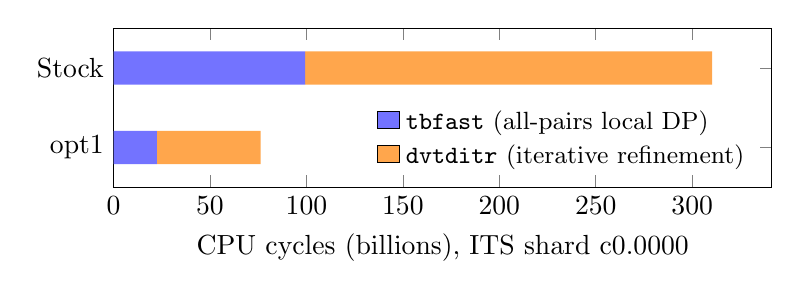
\begin{tikzpicture}
\begin{axis}[
  xbar stacked, width=0.82\linewidth, height=3.6cm,
  xlabel={CPU cycles (billions), ITS shard c0.0000},
  symbolic y coords={opt1,Stock}, ytick=data,
  bar width=12pt, xmin=0,
  legend style={at={(0.98,0.05)},anchor=south east,font=\small,draw=none,fill=none},
  legend cell align=left, enlarge y limits=0.5,
]
\addplot[fill=blue!55,draw=none] coordinates {(99.3,Stock) (22.4,opt1)};
\addplot[fill=orange!70,draw=none] coordinates {(211.0,Stock) (53.9,opt1)};
\legend{\code{tbfast} (all-pairs local DP), \code{dvtditr} (iterative refinement)}
\end{axis}
\end{tikzpicture}
\caption{Where the L-INS-i cycles went, stock and opt1.}
\end{figure}

The opt1 wall-clock benchmarks (Table~\ref{tab:wall}) compared Homebrew's stock MAFFT 7.526
with that build, on a machine whose only other load was macOS background services (load
average about 4). Every output from both builds was byte-identical to the pipeline's stored
reference alignments.

\begin{table}[h]
\centering
\caption{opt1 wall-clock time, L-INS-i on production ITS shards, \code{-{}-thread 1}.}
\label{tab:wall}
\begin{tabular}{lrrr}
\toprule
Test & Stock 7.526 & opt1 & Speedup \\
\midrule
8 shards, one at a time (total) & 717.9\,s & 186.9\,s & 3.84$\times$ \\
\quad per shard & 74--104\,s & 19--28\,s & 3.71--4.08$\times$ \\
16 shards, 8 concurrent (production setting) & 355.9\,s & 95.2\,s & 3.74$\times$\,$^\dagger$ \\
\bottomrule
\multicolumn{4}{l}{\footnotesize $^\dagger$Load rose during the stock run, so this ratio is
approximate; it agrees with the single-run ratio.}
\end{tabular}
\end{table}

The pipeline's own back-to-back measurements gave 3.56--3.97$\times$.

Table~\ref{tab:wall4} gives the current state, measured on macOS 27 with the same method:
builds alternated shard by shard for single runs, and batch order was alternated at 8-way
concurrency, where we also sampled the CPU used by all other processes and would have
discarded any batch run under significant outside load.

\begin{table}[h]
\centering
\caption{opt4 against stock 7.526 and against opt3, L-INS-i on r2 ITS shards,
\code{-{}-thread 1}, macOS 27. All outputs byte-identical to the stored references.}
\label{tab:wall4}
\begin{tabular}{lrrr}
\toprule
Test & Baseline & opt4 & Ratio \\
\midrule
\multicolumn{4}{l}{\emph{vs.\ stock Homebrew 7.526}} \\
8 shards one at a time, wall & 723.8\,s & 111.7\,s & 6.5$\times$ \\
\quad CPU time & 719.6\,s & 99.3\,s & 7.2$\times$ \\
16 shards 8 concurrent, wall & 285.7\,s & 62.6 / 61.3\,s & 4.6$\times$ \\
\quad CPU time & 2{,}021\,s & 310 / 336\,s & 6.3$\times$ \\
\midrule
\multicolumn{4}{l}{\emph{vs.\ opt3}} \\
8 shards one at a time, wall & 120.6\,s & 113.8\,s & 1.06$\times$ \\
\quad CPU time & 103.4\,s & 102.0\,s & 1.01$\times$ \\
16 shards 8 concurrent, wall & 64.5 / 69.9\,s & 63.3 / 66.9\,s & within noise \\
\bottomrule
\end{tabular}
\end{table}

The gain at 8-way concurrency is smaller than for single runs: the eight processes share one
GPU, half the M1's cores are efficiency cores, and short jobs make a 16-shard batch more
sensitive to how the last few line up. opt4's advantage over opt3 is marginal on this
workload; its GPU stage is faster, but that stage is now a small part of each run. Because
every build is byte-identical, choosing among them is purely a performance question.

At production concurrency a region of 2{,}415 shards now takes about 2.6 hours rather than
the roughly 12 it takes with stock MAFFT at the same concurrency.

\subsection{x86}

The x86 benchmarks used the same discipline as on the M1, with nothing else running on the
instance: builds alternated shard by shard for single runs and batch by batch for concurrent
runs, and a sampler recorded any other CPU use. Production packs four single-threaded
alignments per 4-vCPU instance, so concurrency was four. Table~\ref{tab:x86} gives the
first clean comparison of the gcc builds on the c7i.

\begin{table}[h]
\centering
\caption{opt5 against stock 7.526, both built with gcc, on a c7i.xlarge; L-INS-i,
\code{-{}-thread 1}. All outputs byte-identical to stock.}
\label{tab:x86}
\begin{tabular}{lrrr}
\toprule
Test & Stock & opt5 & Ratio \\
\midrule
4 shards one at a time, total & 328.4\,s & 57.2\,s & 5.75$\times$ \\
\quad per shard & 75--98\,s & 12.0--17.3\,s & \\
16 shards, 4 concurrent & 595 / 589\,s & 106 / 104\,s & 5.6$\times$ \\
\quad throughput & 97 shards/h & 549 shards/h & \\
\midrule
\multicolumn{4}{l}{\emph{All 183 test shards, 4 concurrent, mean wall per shard}$^\dagger$} \\
\quad production shards & 157.6\,s & 28.2\,s & 5.6$\times$ \\
\quad targeted windows (217--532 seqs) & 541\,s & 92.7\,s & 5.8$\times$ \\
\quad current-build shards & 107.5\,s & 21.1\,s & 5.1$\times$ \\
\bottomrule
\multicolumn{4}{l}{\footnotesize $^\dagger$The stock run shared the machine with builds at times,
so its times are slightly inflated.}
\end{tabular}
\end{table}

Table~\ref{tab:x86four} compares all four builds on both instance types, each set measured
within one session. The c7i ran 8--15\% slower in its second session than in its first (the
same opt5 batch took 121\,s against 104--106\,s), presumably for host-level reasons, so builds
are compared only within a session. On both machines clang+FMA is 2--6\% faster than gcc,
for stock and for opt5.

\begin{table}[h]
\centering
\caption{Four builds on two instance types, L-INS-i, \code{-{}-thread 1}: 16 production
shards at 4 concurrent (batch wall time, and throughput), and two shards run singly
(c0.0016 / c0.0017). Every output matched the stock build of the same rounding.}
\label{tab:x86four}
\begin{tabular}{lrrrr}
\toprule
& \multicolumn{2}{c}{Stock 7.526} & \multicolumn{2}{c}{opt5} \\
\cmidrule(lr){2-3}\cmidrule(lr){4-5}
& gcc & clang+FMA & gcc & clang+FMA \\
\midrule
\multicolumn{5}{l}{\emph{c7i.xlarge (2 cores $\times$ 2 hyperthreads)}} \\
16 shards, 4 concurrent & 639\,s & 601\,s & 121\,s & 117\,s \\
\quad throughput (shards/h) & 90 & 96 & 476 & 492 \\
single runs & 82.0 / 108.6\,s & 79.1 / 104.1\,s & 13.4 / 19.3\,s & 13.3 / 18.8\,s \\
\midrule
\multicolumn{5}{l}{\emph{c7a.xlarge (4 cores)}} \\
16 shards, 4 concurrent & 439\,s & 411\,s & 76\,s & 70\,s \\
\quad throughput (shards/h) & 131 & 140 & 758 & 823 \\
single runs & 88.0 / 130.5\,s & 82.8 / 124.9\,s & 12.9 / 18.1\,s & 12.4 / 17.2\,s \\
\bottomrule
\end{tabular}
\end{table}

Single-threaded speed is similar on the two machines: opt5 is slightly faster on the c7a and
stock slightly slower. The c7a's advantage is its four real cores: four concurrent jobs
barely slow each other there, whereas on the c7i two hyperthreads share each core and four
jobs give only about 2.2--2.3 times the throughput of one (approximate, since the single runs
and the batches used different production shards). Over all 183 test shards at four concurrent, opt5-clang took 1{,}082\,s on the c7a and
1{,}845\,s on the c7i. At us-west-2 prices at the time (on-demand \$0.205/h for c7a.xlarge and
\$0.1785/h for c7i.xlarge), opt5-clang costs about \$0.25 per 1{,}000 shards on the c7a and
\$0.33--0.36 on the c7i; at a week's range of Spot prices, \$0.11--0.15 and \$0.12--0.20.
The deployment uses the c7a, with the c7i as a Spot fallback, since the two give identical
output. For comparison, opt4 on the M1 aligns about 930 shards per hour at 8 concurrent.

\section{What did not work, and limitations}

\begin{itemize}
\item \textbf{Generality.} The speedups, not the exactness, are specific to this workload and
  hardware. Which optimizations paid depended on the shape of the alignments (about 180
  sequences, about 2{,}000 columns, 71\% gaps), on the default scoring settings, and on the
  machine: banding the importance matrix did not help with a 105\,MB L3 but may with 16\,MB,
  the GPU stage exists only on the Mac, and gains ranged from 5.1$\times$ to 5.8$\times$ across
  our own shard sets at four concurrent. Other inputs or machines may see smaller gains. Every
  fast path checks its preconditions and falls back to the original code, so they will see
  the same output.
\item \textbf{Blocked prefix scan.} Splitting the \code{L\_\_align11} row scan into four
  interleaved chains followed by a fix-up pass was slower when measured side by side
  (28.6G vs.\ 39.2G \code{tbfast} cycles, the latter being the blocked version), and was
  reverted. The added pass and branches cost more than the extra parallelism gained.
\item \textbf{Other scan variants} (Section~\ref{sec:round2}): a scalar next-row scan fused into
  the vector loop, and a two-block unrolled vector scan, were slower or no faster.
\item \textbf{Whole-step memoization in refinement} could reuse at most 2\% of steps, and a
  cache of anchor profiles across FFT lags turned out never to run, since L-INS-i and
  FFT-NS both use MAFFT's single-lag anchoring mode. Both were dropped.
\item \textbf{GPU variant tuning}: finer column-count variants gave nothing; register-resident
  state was a net loss (Table~\ref{tab:occupancy}).
\item \textbf{Scope.} The integer and zero-extension fast paths apply to the default
  scoring settings. Non-default settings, such as fractional \code{-{}-consweight},
  nonzero \code{-{}-gexp} in progressive modes, or \code{-{}-allowshift}, take the original
  code, and are exact but not faster.
\item \textbf{Threads.} We did not make \code{-{}-thread N} deterministic. Stock MAFFT is
  already nondeterministic there, and the pipeline parallelizes across inputs instead.
\item \textbf{Platforms.} NEON, Accelerate and Metal code is guarded by \code{\_\_ARM\_NEON}
  and \code{\_\_APPLE\_\_}, and the x86 kernels by \code{\_\_AVX512F\_\_} (with SSE4.1 versions of
  the local-alignment fill). The AVX-512 build needs \code{-march=x86-64-v4}; without it the
  portable C paths are used, which are exact but were not benchmarked. Graviton (arm64 Linux)
  would take the NEON paths but was not tested; with gcc there, \code{MAFFT\_STOCK\_FMA} would be
  off and the fused NEON row kernels disabled.
\item \textbf{Importance matrix on x86.} Banding the importance-matrix fill and prefetching
  within it did not help on Sapphire Rapids (Section~\ref{sec:opt5}); it remains the largest
  single cost there, and banding was not tried on the c7a's smaller L3.
\item \textbf{Version strings.} The version string does not record the rounding class, so a gcc
  and a clang+FMA build of the same commit cannot be told apart by it
  (Section~\ref{sec:provenance}).
\item \textbf{Trees.} The tree stage is not reproducible across platforms or FastTree builds
  (Section~\ref{sec:xplat}). We did not try to make it so: that would mean building FastTree
  without \code{-funsafe-math-\allowbreak optimizations} on every platform, and would still leave
  differences between the math libraries.
\item \textbf{Coverage.} The corpus the pipeline now aligns on AWS includes ITS sequences up to about
  3{,}000\,bp, longer than anything in the test sets. Those exercise the same code but will cost
  more per shard than the timings here suggest.
\item \textbf{GPU limits.} The GPU takes second sequences of 64--2{,}048 residues; others use
  the CPU. If the embedded shader library fails to load, opt4 silently falls back to
  compiling the source; the only sign is a line on standard error, which MAFFT's
  \code{-{}-quiet} discards.
\end{itemize}

\section{Conclusions}

Mature scientific code can hold large, exact speedups: here 6.5$\times$ on the M1 and
5--7$\times$ on x86, mostly from bookkeeping and data layout rather than new algorithms, and
without changing an output byte, so nothing downstream had to be revalidated. Porting showed
that ``identical to stock'' must name the stock build, because the compiler's rounding of
multiply-adds alone changed a third of the alignments between platforms.

This work was done by an AI coding agent, Claude Code running Claude Opus 5.5, with a
researcher setting the direction and the acceptance rules. It took about a week of calendar
time from the first build to the deployed x86 build, within a \$200/month subscription; by the
authors' estimate the same work would have taken a human developer several weeks. The
compute savings alone repay that slowly: at on-demand prices the x86 build saves about \$1.21
per 1{,}000 shards (\$1.46 against \$0.25 on a c7a), so even charging the whole month to this
work, it is recouped only after about 165{,}000 shards, roughly 70 regions, and after about
twice as many at Spot prices. The immediate return is turnaround: a region that took about 12 hours
to align on the M1 now takes about 2.6, which shortens the research loop.

What made the work safe to delegate was verification, not the agent. The exactness contract
was fixed in advance, each rewritten function was checked against the original on every call,
and a separate Claude Code session working on the pipeline, under its own user's approval,
validated each Mac build on production data before it was installed; the x86 build was
accepted against its reference on the instance types it runs on, and the deployed image
re-runs a canary. The independent check caught the one error the rewrite introduced
(Section~\ref{sec:bug}).

For compute-bound pipelines that run a fixed tool at scale, we therefore recommend profiling
the dominant tool on the hardware it actually runs on and, where results must not change,
attempting exact optimization under the same discipline: an explicit output contract,
per-function bitwise checks, and validation by someone other than the author of the change.

\section{Related work}

SIMD acceleration of pairwise DP is well established. It includes anti-diagonal
vectorization~\cite{wozniak1997}, Farrar's striped layout~\cite{farrar2007}, inter-sequence
parallelism~\cite{rognes2011}, and general libraries such as parasail~\cite{daily2016}.
Those methods typically target score-only or database-search settings with standard
affine recurrences. Our case differs in two ways. First, we must reproduce MAFFT's own
recurrence and traceback conventions and its floating-point rounding exactly. Second, the
largest wins came from removing redundant bookkeeping and from recasting reductions as
dense matrix products that run on matrix hardware. Faster DP kernels alone would not have
produced them. GPU implementations of Smith--Waterman are likewise established, usually for database search
with score-only kernels; our kernel instead computes MAFFT's own recurrence and full
traceback, bit-exactly, for all pairs of a set. Approximate alternatives, such as faster MAFFT modes or other
aligners~\cite{vaser2017}, trade accuracy for speed. The downstream measurements cited
in the introduction quantify that trade for this workload. That floating-point results
depend on compiler contraction and optimization flags is well known in principle; what we
add is a measurement of its size for one widely used aligner on real data (a third of
inputs) and a demonstration that matching the contraction rule alone restores identical
output across architectures.

\section{Availability and future work}
\label{sec:avail}

The builds are a linear series of commits on top of upstream GitLab \code{main} (7.526,
including December 2025 commits). They are published, with this report, as the
\code{exact-speedups} branch of an unofficial fork,
\url{https://github.com/joshuaowalker/mafft}, with one tag per build
(\code{v7.526-opt1} to \code{v7.526-opt5}). In total they change 16 files
(+2{,}638/$-$200 lines), all in \code{core/}. opt4 is installed for local projects on the Mac (opt5 is the same
code there); the earlier builds are kept for rollback. On AWS, opt5 runs in a container image
built from these sources: clang 15 with \code{-O3 -march=x86-64-v4 -DMAFFT\_STOCK\_FMA=1}, next
to the clang+FMA stock reference, trimAl 1.5.1, and the bioconda FastTree binary, copied
rather than rebuilt. The opt5 per-call harnesses are in the fork's \code{harness/opt5}
directory as patch scripts. A self-contained
canary checks a build in one command: L-INS-i on the 13 canary windows and the 12 placement
cases against the Mac's stored outputs, plus the tree stage against x86 hashes. It passes on
opt5-clang and on the Mac's opt4, and fails on exactly the five divergent windows when given
the gcc build. The deployed image runs it on AWS Batch. The canary is built from the pipeline's data and is not published.

Promising next steps are:
(i)~the importance-matrix fill, now the largest cost on x86, by banding on machines whose L3
cannot hold the matrix, such as the c7a;
(ii)~recording the rounding class in the version string itself;
(iii)~making the shader fallback observable, or optionally an error;
(iv)~testing the longest ITS sequences the pipeline now aligns;
and (v)~offering these changes to the MAFFT maintainers.

\begin{thebibliography}{99}\small
\bibitem{katoh2002} K.~Katoh, K.~Misawa, K.~Kuma, T.~Miyata. MAFFT: a novel method for
  rapid multiple sequence alignment based on fast Fourier transform.
  \emph{Nucleic Acids Res.} 30:3059--3066, 2002.
\bibitem{katoh2005} K.~Katoh, K.~Kuma, H.~Toh, T.~Miyata. MAFFT version 5: improvement in
  accuracy of multiple sequence alignment. \emph{Nucleic Acids Res.} 33:511--518, 2005.
\bibitem{katoh2013} K.~Katoh, D.~M.~Standley. MAFFT multiple sequence alignment software
  version 7: improvements in performance and usability. \emph{Mol. Biol. Evol.}
  30:772--780, 2013.
\bibitem{price2010} M.~N.~Price, P.~S.~Dehal, A.~P.~Arkin. FastTree 2 -- approximately
  maximum-likelihood trees for large alignments. \emph{PLoS ONE} 5:e9490, 2010.
\bibitem{capella2009} S.~Capella-Guti\'errez, J.~M.~Silla-Mart\'inez, T.~Gabald\'on.
  trimAl: a tool for automated alignment trimming in large-scale phylogenetic analyses.
  \emph{Bioinformatics} 25:1972--1973, 2009.
\bibitem{vaser2017} R.~Vaser, I.~Sovi\'c, N.~Nagarajan, M.~\v{S}iki\'c. Fast and accurate
  de novo genome assembly from long uncorrected reads. \emph{Genome Res.} 27:737--746,
  2017.
\bibitem{wozniak1997} A.~Wozniak. Using video-oriented instructions to speed up sequence
  comparison. \emph{Comput. Appl. Biosci.} 13:145--150, 1997.
\bibitem{farrar2007} M.~Farrar. Striped Smith--Waterman speeds database searches six times
  over other SIMD implementations. \emph{Bioinformatics} 23:156--161, 2007.
\bibitem{rognes2011} T.~Rognes. Faster Smith--Waterman database searches with
  inter-sequence SIMD parallelisation. \emph{BMC Bioinformatics} 12:221, 2011.
\bibitem{daily2016} J.~Daily. Parasail: SIMD C library for global, semi-global, and local
  pairwise sequence alignments. \emph{BMC Bioinformatics} 17:81, 2016.
\end{thebibliography}

\end{document}
